\documentclass{beamer}

\usepackage[latin1]{inputenc}
\usepackage{algorithmic}
\usepackage{amsmath}
\usepackage{graphicx}
\usepackage{verbatim}
\usepackage{hyperref}

\title{Super-Resolution From a Single Image}
\author{Geoffrey Ulman}
\date{April 21, 2012}
\begin{document}

%%%%%%%%%%%%%%%%%%%%%%%%%%%%%%%%%%%%%%%%%%%%%%%%%%%%

\begin{frame}
\titlepage
\end{frame}

%%%%%%%%%%%%%%%%%%%%%%%%%%%%%%%%%%%%%%%%%%%%%%%%%%%%

\begin{frame}{Original Paper}

Super-Resolution From a Single Image

\vspace{1cm}

\emph{Daniel Glasner, Shai Bagon, Michal Irani}

\vspace{1cm}

\url{http://www.wisdom.weizmann.ac.il/~vision/SingleImageSR.html}

\end{frame}

%%%%%%%%%%%%%%%%%%%%%%%%%%%%%%%%%%%%%%%%%%%%%%%%%%%%

\begin{frame}{Multiple Frame Super-Resolution}

\begin{figure}
\centering
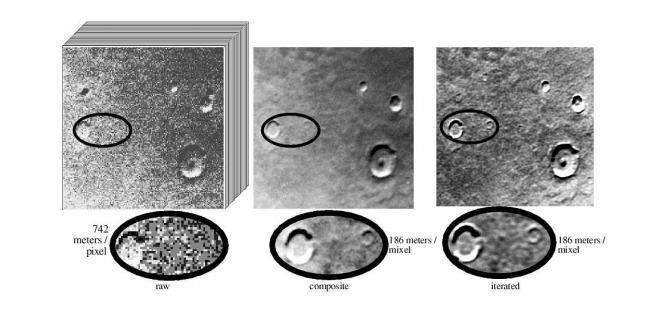
\includegraphics[width=1.0\textwidth]{presentation_screen1.png}
\caption{Multiple images of the same scene with sub-pixel shifts\footnote[1]{\url{http://www.robots.ox.ac.uk/~elle/pubs/elle-thesis.pdf}}}
\end{figure}

\end{frame}


%%%%%%%%%%%%%%%%%%%%%%%%%%%%%%%%%%%%%%%%%%%%%%%%%%%%

\begin{frame}{Multiple Frame Super-Resolution}

Let \( {L_1,...,L_n} \) be a set of images of the same scene.

\vspace{0.3cm}

Assume these images were all derived from a high resolution source image \(H\).

\vspace{0.3cm}

Each low resolution image \(L_j\) was generated by \emph{blurring} and \emph{subsampling} from \(H\).

\vspace{0.3cm}

The \emph{blurring} operation is a convolution with a Gaussian (or similar) kernel \(B_j\).

\begin{figure}
\begin{equation}
\begin{aligned}
L_j = \left( H \otimes B_j \right) \left( q \right) \downarrow s_j
\end{aligned}
\end{equation}
\end{figure}

\end{frame}

%%%%%%%%%%%%%%%%%%%%%%%%%%%%%%%%%%%%%%%%%%%%%%%%%%%%

\begin{frame}{Multiple Frame Super-Resolution}

We can write an equation describing each pixel \(L_j(p)\) of the \(j^{th}\) low resolution image in terms of nearby pixels \(H(q_i)\) in the high resolution image.

\begin{figure}
\begin{equation}
\begin{aligned}
L_j(p) = \sum_{q_i \in Support(B_j)} H( q_i ) B_j( q_i - q )
\end{aligned}
\end{equation}
\end{figure}

For large enough \(j\) this system becomes \emph{over determined} and we can use least squares to approximate the unknown pixels \(H(q)\) in the high resolution image.

\end{frame}

%%%%%%%%%%%%%%%%%%%%%%%%%%%%%%%%%%%%%%%%%%%%%%%%%%%%

\begin{frame}{What If We Only Have One Image?}

\vspace{0.3cm}

Images often contain many similar regions.

\vspace{0.3cm}

\begin{figure}
\centering
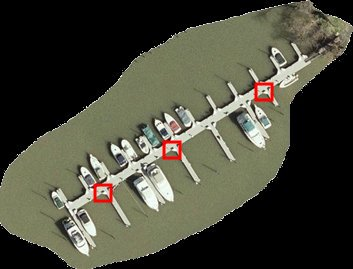
\includegraphics[width=0.7\textwidth]{boatsmall_similar_patches.jpg}
\caption{Similar patches within a single image}
\end{figure}

\end{frame}

%%%%%%%%%%%%%%%%%%%%%%%%%%%%%%%%%%%%%%%%%%%%%%%%%%%%

\begin{frame}{What If We Only Have One Image?}

Break up the problem into many small multiple image super-resolution problems.

\vspace{0.3cm}

For each small patch of the image:

\begin{figure}
\centering
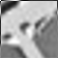
\includegraphics[width=0.1\textwidth]{similar_patches_3.png}
\end{figure}

Search the entire image for similar patches:

\begin{figure}
\centering
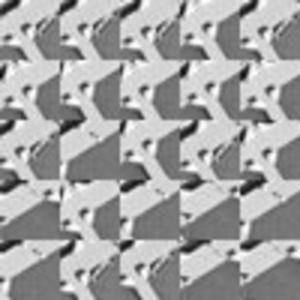
\includegraphics[width=0.35\textwidth]{similar_patches_2.png}
\end{figure}

\end{frame}

%%%%%%%%%%%%%%%%%%%%%%%%%%%%%%%%%%%%%%%%%%%%%%%%%%%%

\begin{frame}{What If We Only Have One Image?}

Now we're back to the multiple image super-resolution formulation (at least for this small portion of the image).

\vspace{0.3cm}

In practice, the patches are quite small ( around 5 by 5 pixels ):

\begin{figure}
\centering
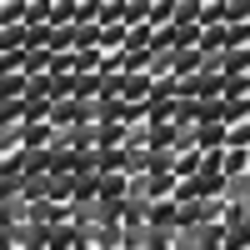
\includegraphics[width=0.5\textwidth]{similar_patches_1.png}
\end{figure}

\end{frame}

%%%%%%%%%%%%%%%%%%%%%%%%%%%%%%%%%%%%%%%%%%%%%%%%%%%%

\begin{frame}{Single Image Super-Resolution Algorithm}

\begin{enumerate}
\item For each pixel in \(L\) find its \(k\) most similar patches
\item Each patch constrains nearby high resolution pixels \(H\)
\item Solve resulting linear system for \(H\)
\end{enumerate}

\end{frame}

%%%%%%%%%%%%%%%%%%%%%%%%%%%%%%%%%%%%%%%%%%%%%%%%%%%%

\begin{frame}[fragile]{Linear System Solvers}

\begin{verbatim}
numpy.linalg.lstsq
\end{verbatim}

\begin{itemize}
\item Return the least-squares solution to a linear matrix equation.

\vspace{0.3cm}

\item Does not allow bounds on independent variables or weights on constraint matrix rows.

\vspace{0.3cm}

\item Very fast even for large problems.

\end{itemize}

\vspace{0.5cm}

\tiny{\url{http://docs.scipy.org/doc/numpy/reference/generated/numpy.linalg.lstsq.html}}

\end{frame}

%%%%%%%%%%%%%%%%%%%%%%%%%%%%%%%%%%%%%%%%%%%%%%%%%%%%

\begin{frame}[fragile]{Linear System Solvers}

\begin{verbatim}
scipy.optimize.nnls
\end{verbatim}

\begin{itemize}
\item Wrapper for FORTRAN non-negative least squares solver.

\vspace{0.3cm}

\item Adds constraint \(x>=0\).

\end{itemize}

\vspace{0.5cm}

\tiny{\url{http://docs.scipy.org/doc/scipy/reference/generated/scipy.optimize.nnls.html}}

\end{frame}

%%%%%%%%%%%%%%%%%%%%%%%%%%%%%%%%%%%%%%%%%%%%%%%%%%%%

\begin{frame}[fragile]{Linear System Solvers}

\begin{verbatim}
scipy.optimize.fmin_slsqp
\end{verbatim}

\begin{itemize}
\item Minimize a function using sequential least squares programming.

\vspace{0.3cm}

\item Allows arbitrary objective function and constraints on independent variables.

\vspace{0.3cm}

\item Was too slow even for small images.

\end{itemize}

\vspace{0.5cm}

\tiny{\url{http://docs.scipy.org/doc/scipy/reference/generated/scipy.optimize.fmin_slsqp.html#scipy.optimize.fmin_slsqp}}

\end{frame}

%%%%%%%%%%%%%%%%%%%%%%%%%%%%%%%%%%%%%%%%%%%%%%%%%%%%

\begin{frame}[fragile]{AMPL Model}

\begin{verbatim}
# output vector (0 to 255 pixel
# values from low resolution image)
param y { 1..l };

# input data
param x { 1..l, 1..n };

# problem variables and simple constraints
# (high definition pixel intensities)
var a {1..n} >= 0, <= 255;

minimize obj: sum { i in 1..l }
                ( ( y[i] - sum { j in 1..n }
                             ( x[i,j] * a[j] ) )^2 );
\end{verbatim}

\end{frame}

%%%%%%%%%%%%%%%%%%%%%%%%%%%%%%%%%%%%%%%%%%%%%%%%%%%%

\begin{frame}[fragile]{Cross-Scale Patch Redundancy}

\begin{figure}
\centering
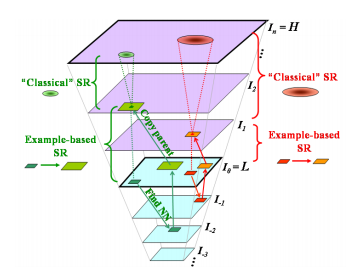
\includegraphics[width=0.6\textwidth]{cross-scale-1.png}
\caption{Multi-Scale Super-Resolution Algorithm\footnote[1]{\url{http://www.wisdom.weizmann.ac.il/~vision/single_image_SR/files/single_image_SR.pdf}}}
\end{figure}

\end{frame}

%%%%%%%%%%%%%%%%%%%%%%%%%%%%%%%%%%%%%%%%%%%%%%%%%%%%

\begin{frame}[fragile]{Cross-Scale Patch Redundancy}

\emph{\Large{Find NN}}

\normalsize

Same as single-scale algorithm, except similar patches are searched for in multiple scaled versions of the low resolution image.

\vspace{0.2cm}

Once found, the similar patch is scaled and pasted into the original low resolution image.

\vspace{0.4cm}

\emph{\Large{Copy Parent}}

\normalsize

The similar patch is used to induce constraints on the high resolution image at the location of the original patch, exactly as with the single-scale algorithm.

\vspace{0.2cm}

The support of the Gaussian kernel must be adjusted for the difference in scale of the similar patch.


\end{frame}

%%%%%%%%%%%%%%%%%%%%%%%%%%%%%%%%%%%%%%%%%%%%%%%%%%%%

\end{document}
